% Options for packages loaded elsewhere
\PassOptionsToPackage{unicode}{hyperref}
\PassOptionsToPackage{hyphens}{url}
%
\documentclass[
]{article}
\usepackage{amsmath,amssymb}
\usepackage{iftex}
\ifPDFTeX
  \usepackage[T1]{fontenc}
  \usepackage[utf8]{inputenc}
  \usepackage{textcomp} % provide euro and other symbols
\else % if luatex or xetex
  \usepackage{unicode-math} % this also loads fontspec
  \defaultfontfeatures{Scale=MatchLowercase}
  \defaultfontfeatures[\rmfamily]{Ligatures=TeX,Scale=1}
\fi
\usepackage{lmodern}
\ifPDFTeX\else
  % xetex/luatex font selection
\fi
% Use upquote if available, for straight quotes in verbatim environments
\IfFileExists{upquote.sty}{\usepackage{upquote}}{}
\IfFileExists{microtype.sty}{% use microtype if available
  \usepackage[]{microtype}
  \UseMicrotypeSet[protrusion]{basicmath} % disable protrusion for tt fonts
}{}
\makeatletter
\@ifundefined{KOMAClassName}{% if non-KOMA class
  \IfFileExists{parskip.sty}{%
    \usepackage{parskip}
  }{% else
    \setlength{\parindent}{0pt}
    \setlength{\parskip}{6pt plus 2pt minus 1pt}}
}{% if KOMA class
  \KOMAoptions{parskip=half}}
\makeatother
\usepackage{xcolor}
\usepackage[margin=1in]{geometry}
\usepackage{color}
\usepackage{fancyvrb}
\newcommand{\VerbBar}{|}
\newcommand{\VERB}{\Verb[commandchars=\\\{\}]}
\DefineVerbatimEnvironment{Highlighting}{Verbatim}{commandchars=\\\{\}}
% Add ',fontsize=\small' for more characters per line
\usepackage{framed}
\definecolor{shadecolor}{RGB}{248,248,248}
\newenvironment{Shaded}{\begin{snugshade}}{\end{snugshade}}
\newcommand{\AlertTok}[1]{\textcolor[rgb]{0.94,0.16,0.16}{#1}}
\newcommand{\AnnotationTok}[1]{\textcolor[rgb]{0.56,0.35,0.01}{\textbf{\textit{#1}}}}
\newcommand{\AttributeTok}[1]{\textcolor[rgb]{0.13,0.29,0.53}{#1}}
\newcommand{\BaseNTok}[1]{\textcolor[rgb]{0.00,0.00,0.81}{#1}}
\newcommand{\BuiltInTok}[1]{#1}
\newcommand{\CharTok}[1]{\textcolor[rgb]{0.31,0.60,0.02}{#1}}
\newcommand{\CommentTok}[1]{\textcolor[rgb]{0.56,0.35,0.01}{\textit{#1}}}
\newcommand{\CommentVarTok}[1]{\textcolor[rgb]{0.56,0.35,0.01}{\textbf{\textit{#1}}}}
\newcommand{\ConstantTok}[1]{\textcolor[rgb]{0.56,0.35,0.01}{#1}}
\newcommand{\ControlFlowTok}[1]{\textcolor[rgb]{0.13,0.29,0.53}{\textbf{#1}}}
\newcommand{\DataTypeTok}[1]{\textcolor[rgb]{0.13,0.29,0.53}{#1}}
\newcommand{\DecValTok}[1]{\textcolor[rgb]{0.00,0.00,0.81}{#1}}
\newcommand{\DocumentationTok}[1]{\textcolor[rgb]{0.56,0.35,0.01}{\textbf{\textit{#1}}}}
\newcommand{\ErrorTok}[1]{\textcolor[rgb]{0.64,0.00,0.00}{\textbf{#1}}}
\newcommand{\ExtensionTok}[1]{#1}
\newcommand{\FloatTok}[1]{\textcolor[rgb]{0.00,0.00,0.81}{#1}}
\newcommand{\FunctionTok}[1]{\textcolor[rgb]{0.13,0.29,0.53}{\textbf{#1}}}
\newcommand{\ImportTok}[1]{#1}
\newcommand{\InformationTok}[1]{\textcolor[rgb]{0.56,0.35,0.01}{\textbf{\textit{#1}}}}
\newcommand{\KeywordTok}[1]{\textcolor[rgb]{0.13,0.29,0.53}{\textbf{#1}}}
\newcommand{\NormalTok}[1]{#1}
\newcommand{\OperatorTok}[1]{\textcolor[rgb]{0.81,0.36,0.00}{\textbf{#1}}}
\newcommand{\OtherTok}[1]{\textcolor[rgb]{0.56,0.35,0.01}{#1}}
\newcommand{\PreprocessorTok}[1]{\textcolor[rgb]{0.56,0.35,0.01}{\textit{#1}}}
\newcommand{\RegionMarkerTok}[1]{#1}
\newcommand{\SpecialCharTok}[1]{\textcolor[rgb]{0.81,0.36,0.00}{\textbf{#1}}}
\newcommand{\SpecialStringTok}[1]{\textcolor[rgb]{0.31,0.60,0.02}{#1}}
\newcommand{\StringTok}[1]{\textcolor[rgb]{0.31,0.60,0.02}{#1}}
\newcommand{\VariableTok}[1]{\textcolor[rgb]{0.00,0.00,0.00}{#1}}
\newcommand{\VerbatimStringTok}[1]{\textcolor[rgb]{0.31,0.60,0.02}{#1}}
\newcommand{\WarningTok}[1]{\textcolor[rgb]{0.56,0.35,0.01}{\textbf{\textit{#1}}}}
\usepackage{graphicx}
\makeatletter
\def\maxwidth{\ifdim\Gin@nat@width>\linewidth\linewidth\else\Gin@nat@width\fi}
\def\maxheight{\ifdim\Gin@nat@height>\textheight\textheight\else\Gin@nat@height\fi}
\makeatother
% Scale images if necessary, so that they will not overflow the page
% margins by default, and it is still possible to overwrite the defaults
% using explicit options in \includegraphics[width, height, ...]{}
\setkeys{Gin}{width=\maxwidth,height=\maxheight,keepaspectratio}
% Set default figure placement to htbp
\makeatletter
\def\fps@figure{htbp}
\makeatother
\setlength{\emergencystretch}{3em} % prevent overfull lines
\providecommand{\tightlist}{%
  \setlength{\itemsep}{0pt}\setlength{\parskip}{0pt}}
\setcounter{secnumdepth}{-\maxdimen} % remove section numbering
\usepackage{booktabs}
\usepackage{longtable}
\usepackage{array}
\usepackage{multirow}
\usepackage{wrapfig}
\usepackage{float}
\usepackage{colortbl}
\usepackage{pdflscape}
\usepackage{tabu}
\usepackage{threeparttable}
\usepackage{threeparttablex}
\usepackage[normalem]{ulem}
\usepackage{makecell}
\usepackage{xcolor}
\ifLuaTeX
  \usepackage{selnolig}  % disable illegal ligatures
\fi
\IfFileExists{bookmark.sty}{\usepackage{bookmark}}{\usepackage{hyperref}}
\IfFileExists{xurl.sty}{\usepackage{xurl}}{} % add URL line breaks if available
\urlstyle{same}
\hypersetup{
  pdftitle={DAG},
  pdfauthor={Shadi},
  hidelinks,
  pdfcreator={LaTeX via pandoc}}

\title{DAG}
\author{Shadi}
\date{2023-06-20}

\begin{document}
\maketitle

\hypertarget{causal-structure-discovery}{%
\subsubsection{Causal Structure
Discovery}\label{causal-structure-discovery}}

I utilized causal structure discovery techniques to accurately represent
the data generating process and unveil the underlying causal
relationships among the variables. The causal structure discovery
approach identifies potential causal relationships based on patterns and
dependencies observed in the data. The resulting Directed Acyclic Graph
(DAG) from the causal discovery is capturing the complex interplay
between the variables, accounting for confounding factors and potential
biases, and providing credible evidence for the causal effects of
medicaid expansion on medicaid take-up and uninsured rate.

By utilizing the DAG obtained through the causal discovery approach, I
can conduct backdoor and front door analyses, enabling the
identification of the minimal adjustment set. The minimal adjustment set
represents the smallest subset of variables that must be controled for
to obtain unbiased estimates of causal effects.

In the initial phase of our analysis, a DAG , as shown in Graph 1, was
generated using multiple constraint-based and score-based algorithms
including GDS algorithms, Greedy Equivalence Search (GES), Peter-Clark
(PC) algorithm, and Fast Causal Inferences (FCI). To integrate the
information obtained from these algorithms, following Joe et al.(2023) I
employed a majority voting approach. This involved considering each edge
and determining its presence in the final graph based on whether it
appeared in more than 50\% of the cases, indicating agreement among the
majority of the algorithms.

\begin{center}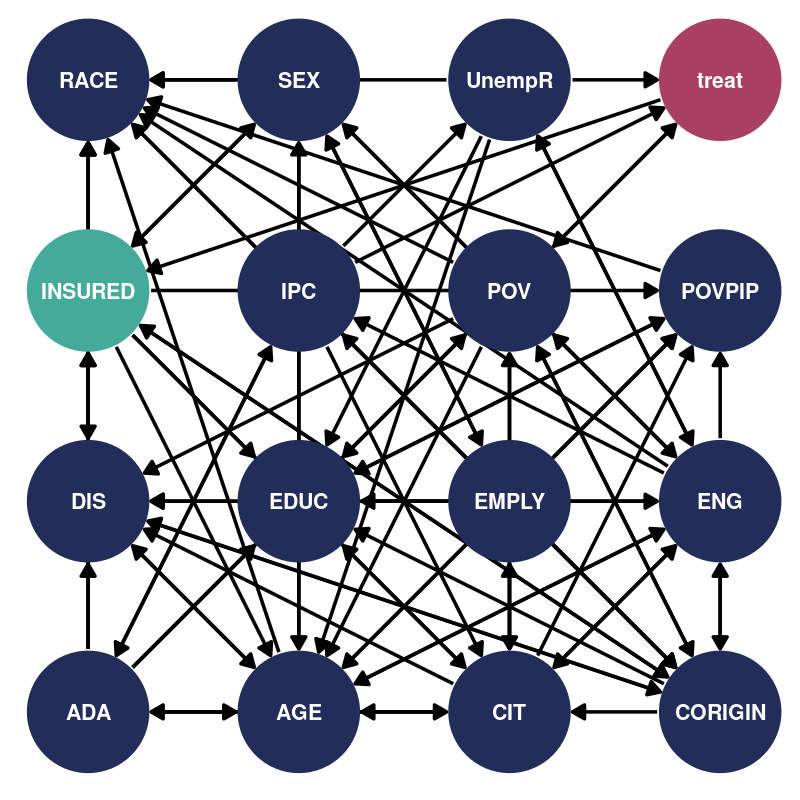
\includegraphics{/home/shadi/Projects/GitHub/medicaid-foreign-born/output/DAG1-1} \end{center}

\hypertarget{revised-casual-graph}{%
\subsubsection{Revised casual graph}\label{revised-casual-graph}}

To enhance the accuracy of the causal relationships represented in the
DAG, I carefully reviewed and manually edited the graph by removing
paths that contradicted my domain knowledge or appeared implausible
within the context. By applying these revisions, the resulting DAG,
illustrated in graph 2, aligns more closely with my expertise in the
field and provides a more trustworthy representation of the underlying
causal structure in my analysis.

\begin{center}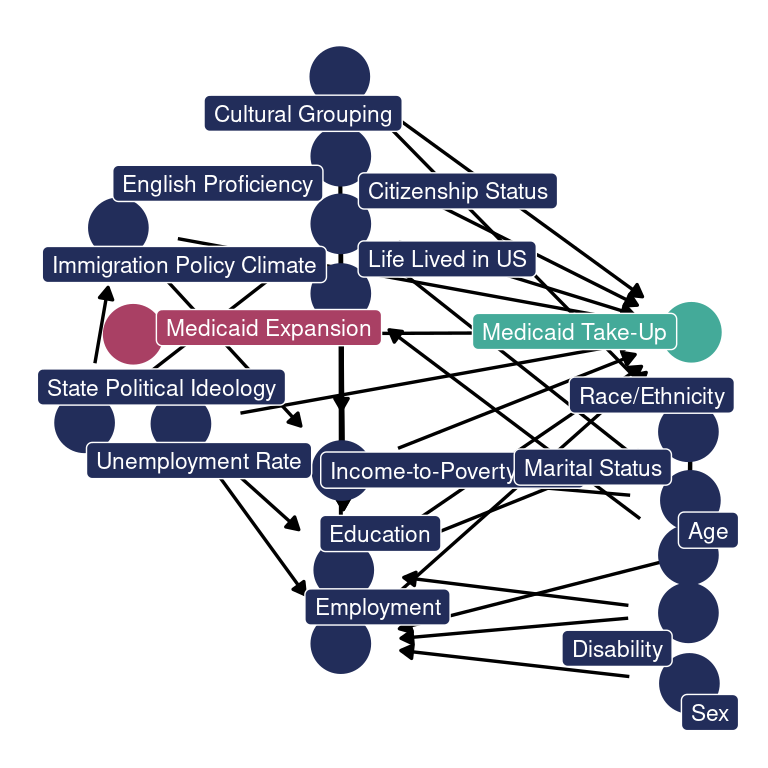
\includegraphics{/home/shadi/Projects/GitHub/medicaid-foreign-born/output/DAG2-1} \end{center}

\hypertarget{minimal-adjustment-set}{%
\subsubsection{Minimal adjustment set}\label{minimal-adjustment-set}}

The identified causal relationship between Medicaid expansion and
Medicaid take-up in the revised DAG provides compelling evidence that
changes in the treatment variable directly influence changes in the
outcome variable. This finding suggests that interventions targeting the
treatment variable, such as expanding Medicaid coverage, can potentially
have a substantial impact on improving the rate of Medicaid take-up.

by conducting backdoor analysis I identified the necessary adjustment
set, revealing that variables Citizenship Status, Immigration Policy
Climate, Unemployment Rate need to be controlled for to accurately
estimate the causal effect between Medicaid expansion and Medicaid
take-up.

\begin{Shaded}
\begin{Highlighting}[]
\FunctionTok{adjustmentSets}\NormalTok{(findag)}
\end{Highlighting}
\end{Shaded}

\begin{verbatim}
## { Citizenship Status, Immigration Policy Climate, Unemployment Rate }
## { State Political Ideology, Unemployment Rate }
\end{verbatim}

\hypertarget{simplified-causal-graph}{%
\subsubsection{Simplified causal graph}\label{simplified-causal-graph}}

To enhance the clarity and interpretability of the graph, I employed a
strategy to simplify its complexity. This involved grouping related
variables into single nodes, such as combining `education,' `income,'
and `employment' into a unified node labeled `Socioeconomic.' The
streamlined representation of the underlying relationships can be
observed in Graph 3.

\begin{center}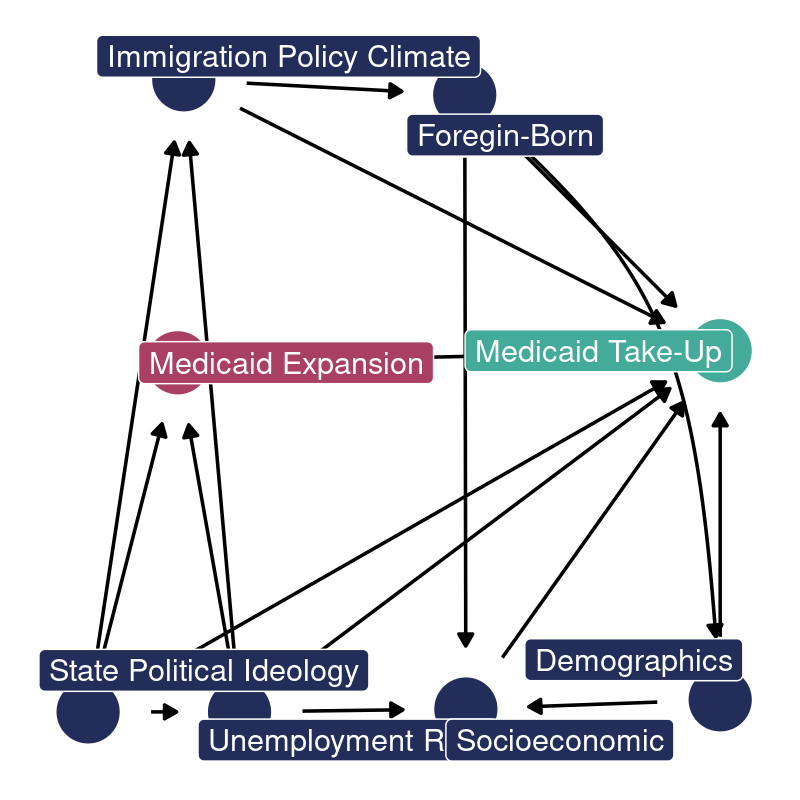
\includegraphics{/home/shadi/Projects/GitHub/medicaid-foreign-born/output/DAG3-1} \end{center}

Although utilizing causal discovery algorithms has limitations, such as
assuming the adequacy of observed variables and relying on the absence
of unobserved confounders, efforts were made to include relevant
variables in the analysis. However, it is possible that unmeasured
confounders may exist, potentially introducing biases into the
identified causal relationships. Therefore, the obtained graph may not
precisely represent the true underlying causal structure..

Due to these limitations, I do not solely rely on this graph and its
suggested adjustment set for estimating causal effects in my analysis.
Nonetheless, the DAG derived from the causal discovery approach serves
as a valuable tool for generating hypotheses and guiding the modeling
process, as well as informing the selection of control variables in my
DID approach analysis.

\end{document}
